\section{Metodologia}

%% ---------------------------------------------------------------------------
% Data Augmentation
\begin{frame}{Data Augmentation (DA)}
    Proposta de duas técnicas de \textit{data augmentation} para gerar AVCDs artificialmente.
    \vspace{0.5cm}

    \begin{itemize}
        \item DA para gerar RIRs simuladas (RIRSM)
        \begin{itemize}
            \item Razão Direto-Reverberante (DRR)
            \item Tempo de Reverberação (T60)
        \end{itemize}
        \item DA para gerar AVCDs, usando RIRSMs e ruídos
    \end{itemize}
    \vspace{0.5cm}

    \begin{figure} 
        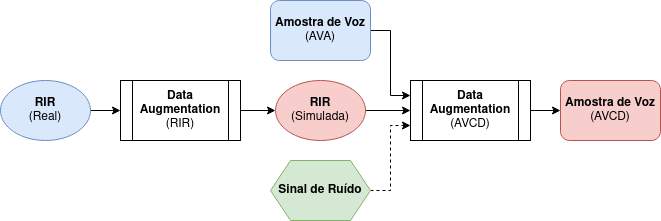
\includegraphics[scale=0.35]{flow-geral.png}
        \label{fig:flow-geral}
    \end{figure}
\end{frame}

\begin{frame}{Data Augmentation (DA)}
    As técnicas de DA de RIRSM e AVCDs foram baseadas, respectivamente, nos artigos abaixo.
    \vspace{0.5cm}
    
    \begin{itemize}
        \item \cite{RIR_Data_Aug} - “Impulse Response Data Augmentation and Deep
        Neural Networks for Blind Room Acoustic Parameter Estimation”
        , N. J. Bryan, ICASSP 2020
        \item \cite{Speech_Rec} - “A study on data augmentation of reverberant speech
        for robust speech recognition”
        , T. Ko et al, ICASSP 2017
    \end{itemize}
\end{frame}

\begin{frame}{Data Augmentation (DA)}
    \begin{align*} 
        h_e(t) &= 
        \begin{cases} 
            h(t), & t_d-t_0 \le t \le t_d+t_0 \\
            0, & \text{caso contrário.}
        \end{cases} \\
        h_l(t) &= 
        \begin{cases} 
            h(t), & t < t_d - t_0 \\
            h(t), & t > t_d + t_0 \\
            0, & \text{caso contrário.}
        \end{cases}
    \end{align*}
    \vspace{0.5cm}

    $h(t) \rightarrow$ RIR \\
    $h_e(t) \rightarrow$ Resposta inicial \\ 
    $h_l(t) \rightarrow$ Resposta atrasada \\
    $t_d \rightarrow$ Tempo levado pelo impulso sonoro da fonte até o receptor \\
    $t_0 \rightarrow$ Janela de tolerância ($t_0 = 2,5$ ms, definido por \cite{RIR_Data_Aug})

\end{frame}

%% ---------------------------------------------------------------------------
% DA - DRR
\begin{frame}{DA - Razão Direto-Reverberante (DRR)}

    Definição do DRR:
    \begin{equation*} 
        DRR_{dB} = 10 \log_{10} \left( \frac{\sum_t h^2_e(t)}{\sum_t h^2_l(t)} \right)
    \end{equation*}
    \vspace{0.5cm}

    DA do DRR:
    \begin{equation*} 
        h'_e(t) = \alpha w_d(t) h_e(t) + [1 - w_d(t)]h_e(t)
    \end{equation*}
    \vspace{0.5cm}

    $w_d(t) \rightarrow$ Janela de Hann de duração $2t_0$
\end{frame}

\begin{frame}{DA - Razão Direto-Reverberante (DRR)}

    Substituindo $h_e(t)$ por $h'_e(t)$ na definição do DRR:
    \begin{equation*}
        \begin{aligned} 
            \alpha^2 \sum_t w^2_d(t) h^2_e(t) +
            2 \alpha \sum_t [1 - w_d(t)] w_d(t) h^2_e(t) + \\
            \sum_t [1 - w_d(t)]^2 h^2_e(t) -
            10^{DRR_{dB}/10} \sum_t h^2_l(t)
            = 0
        \end{aligned}
    \end{equation*}
    \vspace{0.5cm}

    O parâmetro $\alpha$ desejado é a raiz de maior valor.
    
\end{frame}

%% ---------------------------------------------------------------------------
% DA - T60
\begin{frame}{DA - Tempo de Reverberação (T60)}
    Definição do T60:
    \begin{align*}
        \begin{cases}
            t_i, \ \text{onde} \ h(t_i) = max(h(t)) \\
            t_f, \ \text{onde} \ 10 \log_{10} \left( h^2(t_i) - h^2(t_f) \right) = 60 \text{dB} \\
            \text{T60} = t_f-t_i
        \end{cases}
    \end{align*}
    \vspace{0.1cm}

    Modelo de $h_l(t)$:
    \begin{equation*}
        h_m(t) = A e^{-(t - t_o)/ \tau} n(t) u(t - t_o) + \sigma n(t)
    \end{equation*}
    \vspace{0.1cm}

    $A \rightarrow$ Ganho da RIR \\
    $\tau \rightarrow$ Taxa de decaimento \\
    $\sigma \rightarrow$ Desvio padrão do ruído de chão \\
    $n(t) \rightarrow$ Ruído gaussiano padrão \\
    $t_o \rightarrow$ Balor temporal onde $h_l(t)$ tem seu primeiro valor não nulo \\
    $u(t) \rightarrow$ Degrau unitário \\

\end{frame}

\begin{frame}{DA - Tempo de Reverberação (T60)}
    Taxa de decaimento:
    \begin{equation*}
        T60 = \ln(1000) \tau T_s
    \end{equation*}
    \vspace{0.3cm}
    $T_s \rightarrow$ Tempo de amostragem \\

    \vspace{0.3cm}
    DA do T60:
    \begin{equation*}
        h'_l(t) = h_l(t) e^{-(t - t_o) \frac{\tau - \tau_d}{ \tau \tau_d} }
    \end{equation*}
    \vspace{0.3cm}
    
    RIRSM completa:
    \begin{equation*}
        h'(t) = h'_e(t) + h'_l(t)
    \end{equation*}

\end{frame}

%% ---------------------------------------------------------------------------
% DA - AVCD

\begin{frame}{DA - Amostra de Voz em Campo Distante (AVCD)}
    \begin{figure} 
        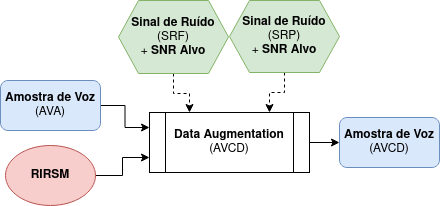
\includegraphics[scale=0.3]{flow-voz-aug.png}
        \label{fig:flow-voz-aug}
    \end{figure}
    \vspace{0.1cm}

    Modelo de uma AVCD:
    \begin{equation*} \label{eqn:AVCD-model}
        S_{cd}[t] = S_a[t] \ast h[t] + \sum_i n_{pi}[t] \ast h[t] + n_f[t]
    \end{equation*}
    \vspace{0.5cm}

    $S_a[t] \rightarrow$ Amostra de Voz Anecóica (AVA) \\
    $h[t] \rightarrow$ RIRSM \\
    $n_p[t] \rightarrow$ Sinal de Ruído Pontual (SRP) \\
    $n_f[t] \rightarrow$ Sinal de Ruído de Fundo (SRF) \\
\end{frame}

\begin{frame}{DA - Amostra de Voz em Campo Distante (AVCD)}
    \textbf{Primeira etapa}: Adição do SRP \\
    \begin{equation*}
        S_r[t] =  S_a[t] \ast h[t] + \alpha \text{ offset}(n_{pi}[t] \ast h[t], o_t)    
    \end{equation*}
    \vspace{0.5cm}

    \textbf{OBS}: $SNR_t = SNR(S_r[t], \alpha (n_{pi}[t] \ast h[t])) \rightarrow$ Razão Sinal-Ruído alvo
    \vspace{0.5cm}

    $S_a[t] \rightarrow$ Amostra de Voz Anecóica (AVA) \\
    $h[t] \rightarrow$ RIRSM \\ 
    $n_{pi}[t] \rightarrow$ SRP \\ 
    $\alpha \rightarrow$ Fator de correção da intensidade de $n_{pi}[t]$ para obter o $SNR_t$ \\
    $\text{offset}(X, o_t) \rightarrow$ Deslocamento de X para uma posição dentro do intervalo de $S_a[t]$ \\
\end{frame}

\begin{frame}{DA - Amostra de Voz em Campo Distante (AVCD)}
    \textbf{Segunda etapa}: Adição do SRF \\
    \begin{equation*}
        S_{cd}[t] =  S_r[t] + \alpha n_f[t]
    \end{equation*}
    \vspace{0.5cm}

    \textbf{OBS}: $SNR_t = SNR(S_{cd}[t], \alpha n_f[t]) \rightarrow$ Razão Sinal-Ruído alvo
    \vspace{0.5cm}

    $S_r[t] \rightarrow$ Amostra de Voz Reverberada + SRP \\
    $n_f[t] \rightarrow$ SRF \\ 
\end{frame}

